\chapter{Results \& Discussion}
\lhead{\emph{Results \& Discussion}} 
\label{chap:discussion}

In order to add stochasticity to the learning, $arm3$ is controlled by a scripted agent. When $agent_{arm3}$ has the ability to transport a cube, it will do so with 50\% chance. 

%This approach strengthens the assumption that the different agents can not find an hidden synchronisation mechanism beside the communication.

\section{Learning approach comparison} 

Table~\ref{tab:exp-0-comparison} demonstrates the veracity of the assumption made in the introduction. The best hyperparameters are used for the training. The best hyperparameters are selected by looking at which parameters maximise $\frac{\textit{ratio of sinked cube}}{\textit{ratio of dropped cube}}$. The simulated problem can be solved optimally when the agents have full observability in a reliable manner. The learning can then be done in a centralised ($CFO$) or decentralised ($DFO$) manner. Removing the agent's access to the full observability of the environment makes the problem unsolvable ($DLO$). Figure~\ref{fig:exp-0-comparision} also shows that with $DLO$ learning, the agents have a tendency to transport cubes even though they do not have certainty about the outcome of their action. This behaviour is studied in-depth in section~\ref{sec:risk-aversion}. Also, table~\ref{tab:exp-0-comparison} confirms that introducing instantaneous communication can help mitigate the partial observability problem ($DLOCI$) and help solving optimally the problem.


\begin{table}[ht]
\centering
\begin{tabular}{lrr}
\toprule
Training method  &            &  Optimality      \\
\midrule
Centralised & $CFO$  & 1.00 \\
Dec. Full obs. &  $DFO$  & 1.00 \\
Dec. Limited obs. & $DLO$  & 0.00 \\
Dec. Limited obs. with delayed com. ($\abs{V}  = 2$) & $DLOCD$ & 0.00 \\
Dec. Limited obs. with instantaneous com. ($\abs{V}  = 2$) & $DLOCI$ & 0.82 \\
\bottomrule
\end{tabular}
\caption[Optimality ratio relative to the training method]{Optimality ratio relative to the training method}
\label{tab:exp-0-comparison}
\end{table}


\begin{tabular}{lr}
\toprule
Method         &  Optimality      \\
\midrule
$CFO$  & 1.00 \\
$DFO$  & 1.00 \\
$DLO$  & 0.00 \\
$DLOCI$ & 0.82 \\
\bottomrule
\end{tabular}


\begin{tabular}{lrr}
\toprule
$TBC1$ state & $TBC2$ state & Intent enc.\\
\midrule
Emtpy & Empty & (11)  \\
Emtpy & Full &  (10) \\
Full & Emtpy & (01) \\
Full & Full & (00) \\
\bottomrule
\end{tabular}



\begin{figure}[ht]
\centering
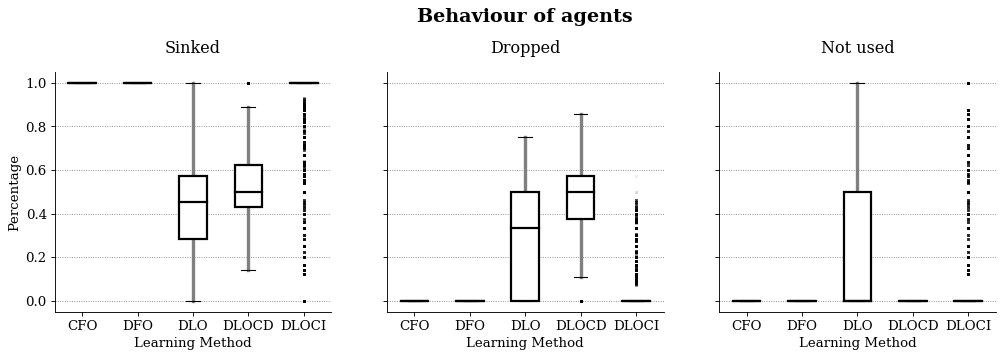
\includegraphics[width=\textwidth]{imgs/exp-0-comparision-fo-lo.png}
\caption[Behaviour of agents relative to training method]{Behaviour of the agents relative to the training method. For each method, the best hyper parameters are used\protect\footnotemark.}
\label{fig:exp-0-comparision}
\end{figure}

\footnotetext{Figure \ref{fig:exp-0-comparision} is constructed from $50$ training session each composed of $500$ evaluation problems. The reparation of cube usage observed in each problem is then aggregated and transcribed in the figure. Hyper parameters used: $CFO$ ($\gamma=0.9$, $r_{time}=-0.1$), $DFO$ ($\gamma=0.9$, $r_{time}=-0.1$), $DLO$ ($\gamma=0.9$, $r_{time}=0.0$, $r_{com}=0.0$), $DLOCD$ ($\gamma=0.9$, $r_{time}=-0.1$, $r_{com}=-0.1$), $DLOCI$ ($\gamma=0.9$, $r_{time}=0.0$, $r_{com}=0.0$).}

Interestingly, in the simulated problems, having a delayed communication ($DLOCD$) precludes the learning of optimal solutions. This might be explained by the absence of a direct link between communication and resulting action. With a delayed communication, a received reward at time $t$ might be related to a communication made at time $t-1$. As a result, it is more difficult for the agents to agree on a grounding of the communication. \cite{foerster_learning_2016} relies on centralised learning and decentralised execution to mitigate this problem. This approach to MARL being out of the scope of this work, instantaneous communication is used in the following analysis.

In order for the agent to have an incentive to transport cubes and to take into account their past action, a time-reward of $-0.1$ and a discount factor of $0.9$ will be used as default values in the subsequent parts of the discussion. 

\section{Risk aversion}
\label{sec:risk-aversion}
When communication is not available and control is decentralised, agents must take action with a much higher degree of uncertainty. The uncertainty raises from the absence of state information about the tail buffer of the conveyors for $agent_{arm1}$ and $agent_{arm2}$.  In the $DLO$ scenario, no optimal solutions are found and a certain number of solutions results in drop of cubes. As reflected in figure~\ref{fig:exp-0-comparision}, they still have a tendency to transport cubes without the guarantee of a positive outcome. 

In a specific training session, an agent is considered to be \textit{risk averse} if it does not perform any other action than $noop$ and \textit{risk seeking} otherwise. The risk aversion of an agent can be seen as a measure of the trade -off between selecting an action with an unknown payoff compared to another one with a possibly lower, but more predictable payoff. 

The $DLO$ setting is particularly suited to study the risk aversion of the agents. Indeed, in this setting both $agent_{arm1}$ and $agent_{arm2}$ have no opportunity to coordinate with respect to the state of the tail buffer of the conveyors. Figures~\ref{fig:exp-1-risk-rwdt} and \ref{fig:exp-1-risk-disc} show the average risk aversion. The risk aversion is calculated by looking at the learned behaviour of both $agent_{arm1}$ and $agent_{arm2}$. The risk aversion represents the ratio of solutions where both agents are risk averse, i.e do not transport any cubes. A risk aversion of $1$ means that in 100\% of the training sessions, both  $agent_{arm1}$ and $agent_{arm2}$ learned to not transport cubes. On the other hand, a risk aversion of $0$ indicates that in all the training sessions both agents were risk seeking and learned to send cube under uncertainty.

\begin{figure}[H]
\centering
\begin{minipage}[t]{.5\textwidth}
  \centering
  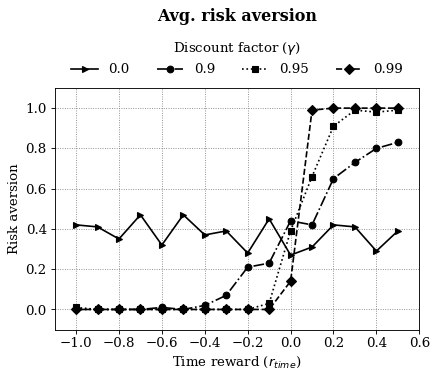
\includegraphics[width=\linewidth]{imgs/exp-1-risk-rwdt.png}
  \caption[Average risk aversion relative to the time-reward]{Average risk aversion relative to the time-reward.}
  \label{fig:exp-1-risk-rwdt}
\end{minipage}%
\begin{minipage}[t]{.5\textwidth}
  \centering
  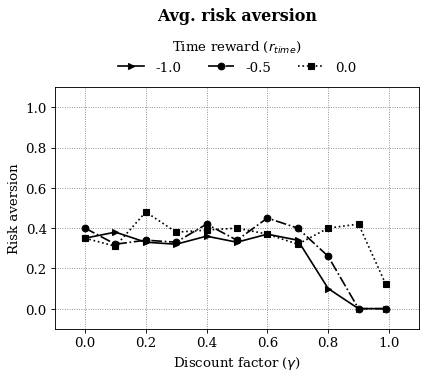
\includegraphics[width=\linewidth]{imgs/exp-1-risk-disc.png}
  \caption[Average risk aversion relative to the discount factor]{Average risk aversion relative to the discount factor.}
  \label{fig:exp-1-risk-disc} 
\end{minipage}
\end{figure}

Acting as a sanity check, when both the time reward and the discount factor are bigger than $0$ the agents have a high risk aversion. The positive time reward pushes the arm to "run the clock". By not transporting any cube, they wait until the maximum number of time steps is reached and as a result maximise the long term return. On the other hand, as long as the agent's horizon is not too long, the time reward does not seem to influence the risk aversion (fig.~\ref{fig:exp-1-risk-disc}). At the extreme, the discount factor of $0$  the time reward only shifts all Q estimates by the same amount. As the discount factor gets closer to 1, the arms become more risk seeking. With the goal of maximising the long term reward, any transported cube will make the episode finish faster. In addition to shortening the episode, a few cubes might be transported correctly which increases the total long term reward. 

%%%%%%%%%%%%%%%%%%%%%%%%%%%%%%%%%%%%%%%%%%%%%%%%%%%%%%
%%%%%%%%%%%%%%%%%%%%%%%%%%%%%%%%%%%%%%%%%%%%%%%%%%%%%%
%%%%%%%%%%%%%%%%%%%%%%%%%%%%%%%%%%%%%%%%%%%%%%%%%%%%%%
%%%%%%%%%%%%%%%%%%%%%%%%%%%%%%%%%%%%%%%%%%%%%%%%%%%%%%

\section{Communication Analysis}

\subsection{Influence of communication reward}

The cost related to the channel usage is introduced by adding a communication reward to the global reward for $agent_{arm3c}$. As explained in section \ref{sec:reward-function}, the communication reward is only added to the sender. As a reminder, the messages in the vocabulary from which the communication agent picks are labelled from $0$ to $\abs{V} - 1$. The usage of the message $v_0$ incurs no cost as it is the equivalent to "no message sent". In order to facilitate the analysis of the influence of the communication reward in the $DLOCI$, a vocabulary of size $2$ is used. 

\begin{figure}[H]
\centering
\begin{minipage}[t]{.5\textwidth}
    \centering
    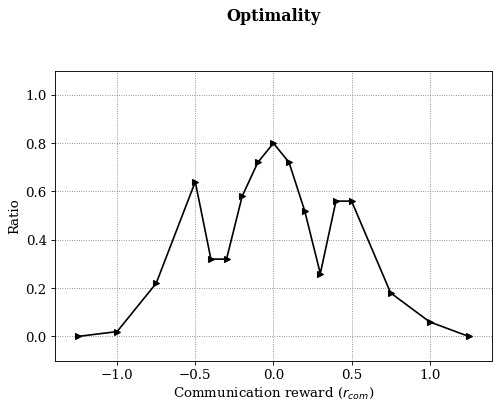
\includegraphics[width=0.95\textwidth]{imgs/exp-2-rwdc-2msg-optimality.png}
    \caption[Influence of $r_{com}$ on optimality of learning]{Optimality of learning when trained with hyperparameters $\abs{V}=2$, $r_{time}=-0.1$ and $\gamma=0.9$ relative to the cost of communication.}
    \label{fig:exp-2-rwdc-optimal}
\end{minipage}%
\begin{minipage}[t]{.50\textwidth}
    \centering
    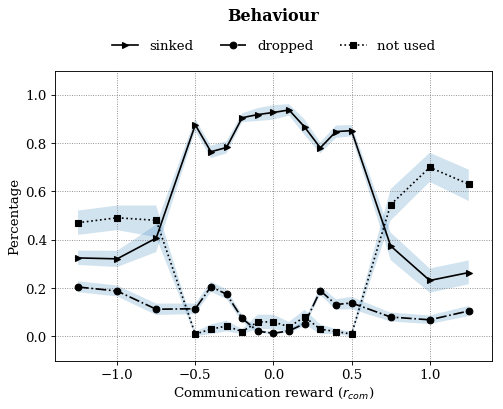
\includegraphics[width=0.95\textwidth]{imgs/exp-2-rwdc-2msg-behaviour.png}
    \caption[Influence of $r_{com}$ on the behaviour of the agents]{Behaviour of the agents when trained with hyperparameters $\abs{V}=2$, $r_{time}=-0.1$ and $\gamma=0.9$ relative to the cost of communication.}
    \label{fig:exp-2-rwdc-behaviour}
\end{minipage}
\end{figure}

Figures~\ref{fig:exp-2-rwdc-optimal} and \ref{fig:exp-2-rwdc-behaviour} shows that the ratio of optimal solution drops to 0 when the absolute value of the communication reward is too high. With such a communication reward, the agents reach a sub-optimal Nash equilibrium. $Agent_{arm3c}$ will learn to always send a specific message from the vocabulary depending on the sign of the communication reward. It will do so in order to maximise its own reward. Following convergence, an improvement in the solution can only be expected if all agents change their behaviour. One can see that with only two messages available the most reliable learning is done with a cost-less or an almost cost-less communication channel (i.e. $r_{com}\approx0$). With no implicit constraint on the usage of the vocabulary there is a higher chance than the agents will converge to a optimal solution. The behaviour is similar for $\abs{v}=4$ when $t_{com} \leq 0$. When $t_{com} > 0$, the drop in optimality is not seen. Indeed, $agent_{arm3c}$ can now discard the use of $v_0$ and still have access to a sufficient vocabulary size to solve the problem optimally.

%\todo{Dip of the optimality around +- 0.25 => why?}

\subsubsection*{Grounding of communication}

Grounding of communication between interacting entities is a widely researched topic. First introduced by Clark, Herbert H. and Brennan, Susan E. (1991) \cite{resnick_grounding_1991}, it relates to the collection of "mutual knowledge, mutual beliefs, and mutual assumptions" that is required for successful communication between two entities. A common grounding criterion is that everyone involved has a clear enough understanding of the concept and intent transported through the communication channel to move forward correctly \cite{horvitz_grounding_2000}. Also, in the setting of reinforcement learning, a link with the \textit{new contribution} method proposed by \cite{clark_contributing_nodate} to reach grounding of communication can be made. This method relies on a partner moving forward with a new idea and waiting to see if its partners expresses confusion. In reinforcement learning, this can be seen as sending a specific message and looking at the resulting reward. The reward then acts as an indication of the confusion of the other agents \cite{koschmann_reconsidering_2003}.

\begin{table}[H]
    \centering
    \begin{tabular}{lrrr}
        \toprule
        $TBC1$ state & $TBC2$ state & Intent enc. & Who can transport safely a cube? \\
        \midrule
        Emtpy & Empty & (11) & Both feeding arms \\
        Emtpy & Full &  (10) & Only $arm1$ \\
        Full & Emtpy & (01) & Only $arm2$ \\
        Full & Full & (00) & Not safe for both \\
        \bottomrule
    \end{tabular}
    \caption[Abstracted sub states for $agent_{arm3c}$]{Abstracted sub states for $agent_{arm3c}$. The sub states represents the possible intents that can be transmitted though the communucation channel.}
    \label{tab:agent3c-substate}
\end{table}

The grounding of communication focuses on the interconnection between the intent of the message sent and its interpretation by the receiving agents. Only protocols resulting in optimal solution will be studied. The protocols are inferred from the learned Q-Table. An optimal solution guarantees that at least one message is sent with the intent to indicate that it is not safe for both agents to transport a cube and interpreted correctly. It is important to note that even tough the intent of a message might be "safe for both", in reality $agent_{arm1}$ interprets this message as "safe for me" as it has no notion of existence of $agent_{arm2}$. The same can be said for the interpretation at $agent_{arm2}$. It is only when looking at the intent of the message and the reaction of both feeding arm to the message that it is possible to determine the overall grounding of the protocol.

The state space of $agent_{arm3c}$ is not limited to the status of the buffer $TBC1$ and $TBC2$. Consequently, the communicating agent could send more than a one symbol per sub state. However, it will have to do it at different time steps. The sub state can be seen as a categorisation on top of the state of $agent_{arm3c}$. For example, $agent_{arm3c}$ can be in sub state $00$ while the underlying arm is moving or not which gives two different states. Also, $agent_{arm3c}$ can send the same message $v$ in different sub states.

The grounding of the communication can be represented by a tripartite graph. Figure~\ref{fig:protocol-2msg-good} depicts an example of such a graph. The nodes on the left side represent the intent of the message sent which is related to the sub states shown in table~\ref{tab:agent3c-substate}. The nodes on the right correspond to the interpretation of the message by $agent_{arm1}$ and $agent_{arm2}$. Both the intent and the interpretation are encoded using a binary representation. A "$1$" indicates "safe to transport" and a "$0$" indicates "not safe to transport". For example, "$10$" on the intent side means that it is safe for $agent_{arm1}$ to transport a cube while it is not for $agent_{arm2}$. On the other hand, "$10$" on the interpretation side means that $agent_{arm1}$ interprets the message as "safe for me to transport" while  $agent_{arm2}$ interprets it as "not safe for me to transport". Finally, the nodes in the middle represent the vocabulary. The example presents a possible grounding of communication leading to an optimal solution when $\abs{V} = 2$. This type of protocol only transmits two intents through the channel: the fact that both feeding arms can send safely as well as the opposite. Each intent correctly transmitted though the channel is represented by a coloured node on both side of the graph. A dashed arrow depicts an intent not correctly interpreted by at least one of the the feeding agents. When the number of intent correctly transmitted is equal to the number of available symbols, the protocol will be called ideal, otherwise non-ideal. 

\begin{figure}[H]
\centering
\begin{minipage}[t]{.5\textwidth}
  \centering
  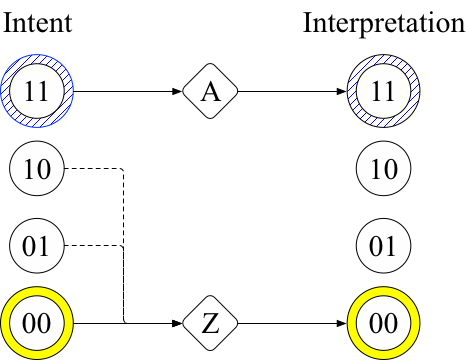
\includegraphics[width=.85\linewidth]{imgs/protocol-2msg-good.png}
  \caption[Ideal protocol for $\abs{V} = 2$]{Example of an ideal protocol for $\abs{V} = 2$ leading to an optimal solution.}
  \label{fig:protocol-2msg-good}
\end{minipage}%
\begin{minipage}[t]{.5\textwidth}
  \centering
  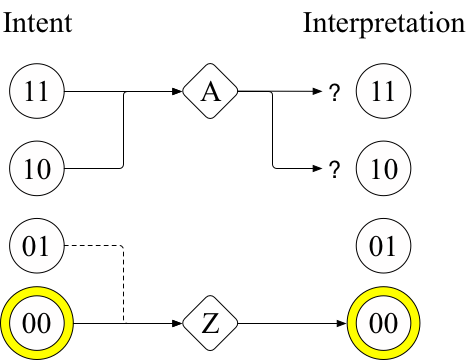
\includegraphics[width=.85\linewidth]{imgs/protocol-2msg-bad.png}
  \caption[Misinterpreted protocol for $\abs{V} = 2$]{Example of protocol for $\abs{V} = 2$ leading to a sub-optimal solution.}
  \label{fig:protocol-2msg-bad}
\end{minipage}
\end{figure}

Out of the 16 possible types of protocol, only five types can lead to an optimal solution (see fig.~\ref{tab:exp-2-assigments-distrib} for the list). In order to distinguish them, a binary encoding of the intents correctly interpreted is used. Each digit of the binary strings of length $4$ represents one of the intent present in table~\ref{tab:agent3c-substate}. If the related intent is correctly transmitted and interpreted, a $1$ will be present in the encoding, otherwise $0$ is used. The example above thus result in the encoding $1001$. We distinguish between the protocol type and the protocol itself. A protocol type indicates which intent is correctly interpreted. On the other hand, a protocol is a realisation of a protocol type where the symbols of the vocabulary have been assigned to a specific vocabulary node in the graph.

It is clear that with a vocabulary of size $2$ the only grounding leading to an optimal solution is based on the protocol type $1001$.  As a result, there exists only two valid protocols and both are ideal protocols. A valid protocol is a protocol leading to an optimal solution. They correspond to the two different assignments of the symbols of the vocabulary to the node $A$ and $Z$. One where the symbol $v_1$ is assigned to node $A$ and $v_0$ to node $Z$ and the opposite. Figure~\ref{fig:protocol-2msg-bad} depicts an invalid protocol. Compared to before, $agent_{arm3c}$ also tries to convey information about the sub sate "safe for $arm1$ but not safe for $arm2$" via symbol $A$. Because of this change in the protocol, it is now impossible for $agent_{arm2}$ to decipher whether it is safe to transport a cube or not. For $agent_{arm2}$, symbol $A$ now indicates that $TBC2$ can either be full or empty. As a result $agent_{arm2}$ can no longer definitively know the intent conveyed by $A$. In this situation, $agent_{arm2}$ can not know the state of $TBC2$ with certainty. As a result will either learn to not send any cube or send cube by becoming risk seeking. Either way, this will result into a non optimal solution with less than 100\% of the cube sinked.

\subsubsection*{Influence of communication-reward on the grounding of communication}

When looking at optimal solutions with a vocabulary of size $2$ $V = (v_0, v_1)$ over a perfect channel,  the communication reward influences the meaning that the agents agree to attribute to specific symbols (fig.~\ref{fig:exp-2-rwdc}). When the cost of using the channel is greater than $0$, the communicating agent has an incentive to use the costly message ($v_1$) when there are no possibilities of receiving any other positive reward. As a result, $v_1$ will be used to indicate the intent "$00$" (i.e. "not safe to transport for both"). On the other hand, when the cost is lower than $0$, the inverse happens. The agents will converge to a grounding of the communication using the costly message ($v_1$) to indicate that both feeding arms can transport cube safely. The positive reward received after a successful transport is used to compensate the usage cost of the channel. When there is no cost in using either word of the vocabulary, no preference in the grounding of the protocol is seen. Half the time the costly symbol will convey information that will push the feeding agents to transport and the other half will indicate they should not move.

\begin{figure}[H]
\centering
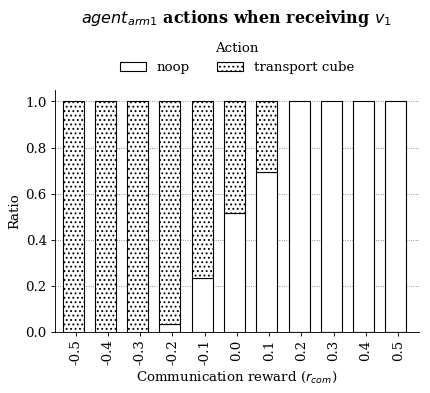
\includegraphics[width=0.5\textwidth]{imgs/exp-2-rwdc-2msg-grounding-a1.png}
\caption[Grounding of communication relative to $r_{com}$ for \abs{v}=2]{$agent_{arm1}$ reaction to receiving message $v_1$. Only looks at state where $agent_{arm1}$ could potentially transport a cube.}
\label{fig:exp-2-rwdc}
\end{figure}

%%%%%%%%%%%%%%%%%%%%%%%%%%%%%%%%%%%%%%%%%%%%%%%%%%%%%%
%%%%%%%%%%%%%%%%%%%%%%%%%%%%%%%%%%%%%%%%%%%%%%%%%%%%%%
%%%%%%%%%%%%%%%%%%%%%%%%%%%%%%%%%%%%%%%%%%%%%%%%%%%%%%
%%%%%%%%%%%%%%%%%%%%%%%%%%%%%%%%%%%%%%%%%%%%%%%%%%%%%%

\subsection{Vocabulary size}

Until now, only solutions with the minimum amount of symbols necessary to solve the task were considered. As shown before, not all possible protocol graphs and assignments of the vocabulary can lead to an optimal solution and considered valid. The number of valid protocols relative to the size of the vocabulary is shown in table~\ref{tab:exp-2-assigments}. 

\begin{table}[H]
\centering
\begin{minipage}[t]{.5\textwidth}
    \centering
    \begin{tabular}{lrr}
    \toprule
    $\abs{V} $ & \multicolumn{2}{c}{Valid assignments} \\
    \midrule
    $2$ & 12.5\% & (2/16)\\
    $3$ & 37.5\% & (24/64)\\
    $4$ & 57.8\% & (146/256)\\
    $8$ & 89.2\% & (58466/65536)\\
    \bottomrule
    \end{tabular}
    \caption[Number of valid vocabulary assignments]{Number of valid vocabulary assignments relative to the size of the vocabulary. Representation: (valid protocols/ possible protocols)}.
    \label{tab:exp-2-assigments}
\end{minipage}%
\begin{minipage}[t]{.50\textwidth}
    \centering
    \begin{tabular}{lr}
    \toprule
    $\abs{V} $ &  optimality \\
    \midrule
    2.0 &   0.78 \\
    3.0 &   1.00 \\
    4.0 &   0.94 \\
    8.0 &   0.96 \\
    \bottomrule
    \end{tabular}
    \caption[Optimality ratios with default hyperparameters relative to vocabulary size]{Optimality ratio for 50 training session with hyperparameters $r_{time}=-0.1$, $r_{com}=-0.1$ and $\gamma=0.9$}
    \label{tab:exp-2-vocabulary-optimal}
\end{minipage}
\end{table}

As shown in table~\ref{tab:exp-2-vocabulary-optimal}, the increase in vocabulary size also brings an increase in the probability of getting an optimal solution at the end of a training session. With a bigger vocabulary there is a higher chance to converge to an optimal solution compared to $\abs{V}=2$. For $\abs{V}=2$, a single misinterpretation will make the solution sub-optimal. 

When more than two words are available, most valid protocols can be simplified. Even tough the agents could convey more than two intents through the channel, it is not required to solve the problem optimally. In case the sender is not precise enough or the receivers are not able to learn correctly the intent of each symbol, it might be possible to discard the intent or the symbol altogether.

\subsubsection*{Complexity}

As representation of the complexity of a learned protocol, the number of intents that are correctly interpreted is used. As a result, in order to achieve the maximum complexity the vocabulary needs to be composed of a minimum of 4 symbols. Table~\ref{tab:exp-2-assigments-distrib} shows the different types of protocol and their respective ratio out of the pool of valid protocols \footnote{The assignments are generated using random sampling of possible protocols. Each generated protocol is then checked to see if it can lead to an optimal solution. If it is the case, the type of protocol is then determined.}.


\begin{table}[H]
 \centering
    \begin{tabular}{lrrrr}
    \toprule
    Protocol type & $\abs{V}  = 2$ & $\abs{V}  = 3$ & $\abs{V}  = 4$ & $\abs{V}  = 8$ \\
    \midrule
    $0111$ & 0 & \underline{25\%} & 24.6\% & 9.9\% \\
    $1001$ & \underline{100\%}\ & 25\% & 9.5\% & 9.9\% \\
    $1011$ & 0 & \underline{25\%} & 24.6\% & 4.3\% \\
    $1101$ & 0 & \underline{25\%} & 24.6\% & 9.9\% \\
    $1111$ & 0 & 0 & \underline{16.4\%} &  \underline{69.8\%} \\
    \bottomrule
    \end{tabular}
    \caption[Distribution of protocol type]{Distribution of the type of protocols relative to the vocabulary size. For each vocabulary size, ratios relative to ideal protocols are underlined. }
    \label{tab:exp-2-assigments-distrib}
\end{table}

Figure~\ref{fig:exp-2-assigments} shows that even though the vocabulary size increases, it is not guaranteed that the learned protocol will be complex or ideal. Also, the agents do not ground the learned protocols uniformly. In most of the training sessions, the intent conveyed by the learned protocol is limited to $01$, $10$ and $11$ (protocol $0111$). 

\begin{figure}[H]
\centering
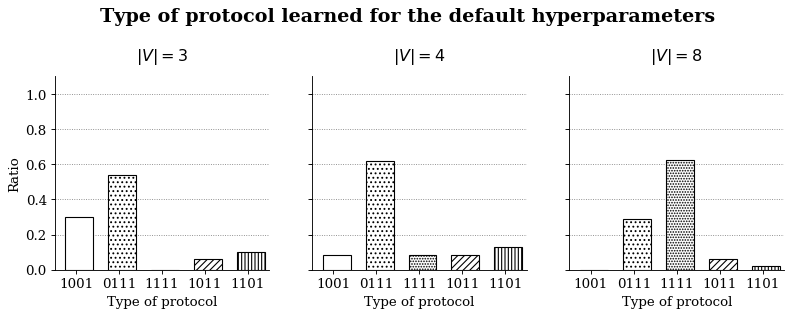
\includegraphics[width=\textwidth]{imgs/exp-2-complexity-default-comparison.png}
\caption[Empirical distribution of protocol types (default parameters)]{Empirical distribution of protocol types for 50 training sessions with hyperparameter $r_{time}=-0.1$, $r_{com}=-0.1$, $\gamma=0.9$}
\label{fig:exp-2-assigments}
\end{figure}

The protocols have thus a tendency to only convey individual safety intent except when the vocabulary size is greater than the number of possible intents. In this setting, the protocol is more often ideal (indicates all intents, i.e. protocol type $1111$). This behaviour can probably be attributed to the fact that the protocol $1111$ is the most common assignment for $\abs{V} = 8$.

An example of a learned protocol with a non-ideal usage of a vocabulary of size $4$ is depicted in \ref{fig:protocol-4msg-bad}. In this example $agent_{arm3c}$ tries to convey to two intents via symbol $A$. Contrary to $agent_{arm2}$, $agent_{arm1}$ can correctly interpret symbol $A$. For $agent_{arm1}$, the symbol $A$ always indicate that it is safe to transport a cube. On the other hand, symbol $A$ conveys two contradictory intents to $agent_{arm2}$ and as a result the agent will not be able to leverage the received communication for its decision process. An ideal protocol with 4 messages can be found in figure~\ref{fig:protocol-4msg-good}. With such protocol, all messages indicate a different sub state and the vocabulary is maximally used.

\begin{figure}[H]
\centering
\begin{minipage}[t]{.5\textwidth}
    \centering
    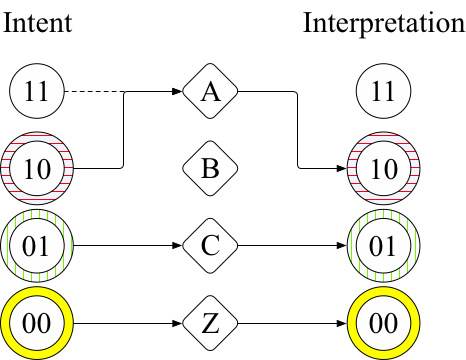
\includegraphics[width=0.95\textwidth]{imgs/protocol-4msg-low.png}
    \caption[Non-ideal communication protocol for $\abs{V} = 4$]{Non-ideal communication protocol for $\abs{V} = 4$ (protocol type : $0111$)}
    \label{fig:protocol-4msg-bad}
\end{minipage}%
\begin{minipage}[t]{.50\textwidth}
    \centering
    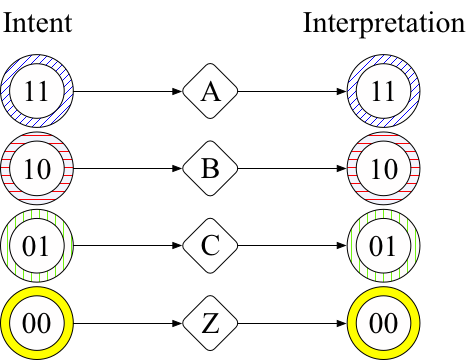
\includegraphics[width=0.95\textwidth]{imgs/protocol-4msg-high.png}
    \caption[Ideal communication protocol for $\abs{V} = 4$]{Ideal communication protocol for $\abs{V} = 4$ (protocol type : $1111$)}
    \label{fig:protocol-4msg-good}
\end{minipage}
\end{figure}

\subsubsection*{Influence of the discount factor on complexity}

The ratio of solutions with an ideal protocol (fig.~\ref{fig:exp-2-disc}) can be increased by lowering the discount factor. By being myopic, the goal is to receive a positive reward as often as possible. In our experiments, a positive reward is received each time a cube is transported correctly. As a result, a low discount rate pushes $agent_{arm3c}$ to indicate as soon as possible an empty buffer. Also, the grounding of communication is facilitated as the estimated Q function contains less noise coming from decisions made in different states. At the extreme, with a discount rate of 0, the agents receive a direct feedback about the quality of the communication. This increase is visible for all vocabulary size as shown in figure~\ref{fig:exp-2-disc-best}.

%\todo{justify parameter selection for gamma}

\begin{figure}[ht]
\centering
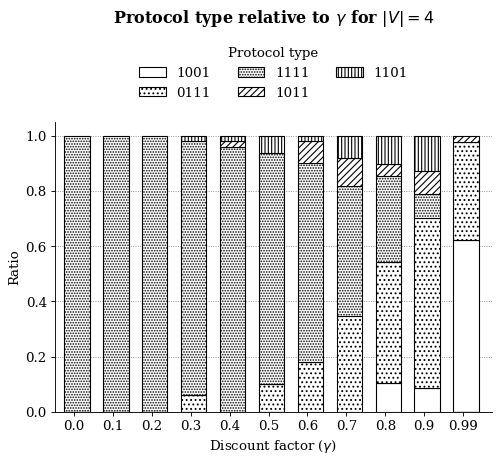
\includegraphics[width=0.6\textwidth]{imgs/exp-2-complexity-4msgs-discount.png}
\caption[Empirical distribution of protocol types relative to the discount rate]{Distribution of protocol types relative to the discount rate for $\abs{v}=4$.}
\label{fig:exp-2-disc}
\end{figure}

\begin{figure}[ht]
\centering
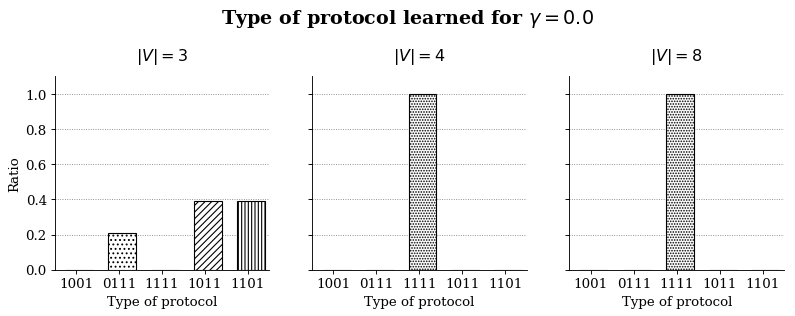
\includegraphics[width=\textwidth]{imgs/exp-2-complexity-best-comparison.png}
\caption[Empirical distribution of protocol types (best parameters)]{Empirical distribution of the protocol type for 50 training sessions with hyperparameter $r_{time}=-0.1$, $r_{com}=-0.1$, $\gamma=0.0$}
\label{fig:exp-2-disc-best}
\end{figure}

% %%%%%%%%%%%%%%%%%%%%%%%%%%%%%%%%%%%%%%%%%%%%%%%%%%%%%%
% %%%%%%%%%%%%%%%%%%%%%%%%%%%%%%%%%%%%%%%%%%%%%%%%%%%%%%
% %%%%%%%%%%%%%%%%%%%%%%%%%%%%%%%%%%%%%%%%%%%%%%%%%%%%%%
% %%%%%%%%%%%%%%%%%%%%%%%%%%%%%%%%%%%%%%%%%%%%%%%%%%%%%%

\section{Unreliable channel}

Up to now, the channel has been assumed to be fully reliable. As a result not sending a message can be seen as a standalone word of the vocabulary. Moving to an unreliable channel which can drop messages introduces a prerogative on the usage of the channel. The message $v_0$ ("no message sent") must now be grounded as intent "$00$" (i.e "not safe for both"). Indeed, if any of the feeding agent ground the communication differently, a dropped message might be misinterpreted and lead to a drop of cube. This behaviour is reflected in figure~\ref{fig:exp-3-grounding}.

\begin{figure}[ht]
\centering
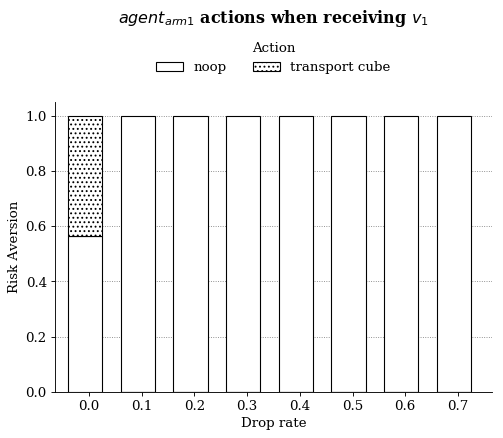
\includegraphics[width=0.5\textwidth]{imgs/exp-3-2msg-grounding-a1.png}
\caption[Reaction to received communication relative to the drop rate]{Reaction to received communication relative to the drop rate.}
\label{fig:exp-3-grounding}
\end{figure}

As shown in table~\ref{tab:exp-3-assigments}, by putting a prerequisite usage of message $0$, the number of possible valid protocols is reduced.  As expected, due to this reduction, the number of optimal solutions is lower. Also, no optimal solutions are found when the drop rate is too high (fig~\ref{fig:exp-3-behaviour}).
\begin{table}[ht]
    \centering
    \begin{tabular}{lrr}
    \toprule
    $\abs{V} $ & \multicolumn{2}{c}{Valid assignment} \\
    \midrule
    $2$ & 6.2\% & (1/16)\\
    $3$ & 14.0 & (9/64) \\
    $4$ & 19.1\% & (49/256)\\
    $8$ & 27.5\% & (16129/58466)\\
    \bottomrule
    \end{tabular}
    \caption[Valid vocabulary assignments with unreliable channel]{Valid vocabulary assignments when channel is unreliable. This channel requires the $v_0$ to convey intent $00$.}
    \label{tab:exp-3-assigments}
\end{table}


\begin{figure}[ht]
\centering
\begin{minipage}[t]{.5\textwidth}
    \centering
    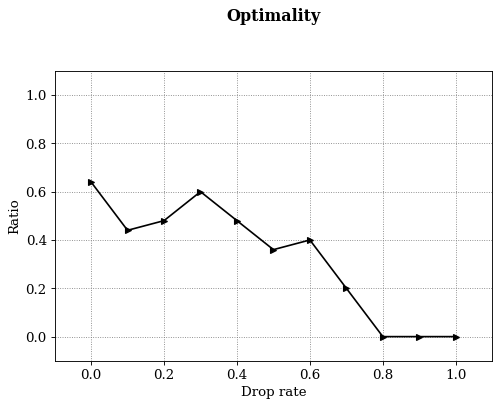
\includegraphics[width=0.95\textwidth]{imgs/exp-3-2msg-optimality.png}
    \caption[Optimality relative to the drop rate]{Optimality of learning relative to the drop rate.}
    \label{fig:exp-3-behaviour}
\end{minipage}%
% \begin{minipage}[t]{.50\textwidth}
%     \centering
%     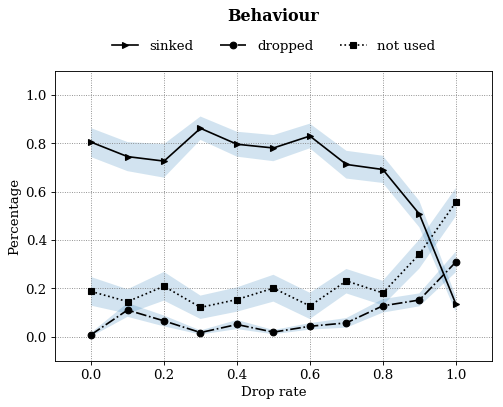
\includegraphics[width=0.95\textwidth]{imgs/exp-3-2msg-behaviour.png}
%     \caption[Behaviour of agents relative to the drop rate]{Behaviour of agents relative to the drop rate.}
%     \label{fig:protocol-4msg-good}
% \end{minipage}
\end{figure}


% %%%%%%%%%%%%%%%%%%%%%%%%%%%%%%%%%%%%%%%%%%%%%%%%%%%%%%
% %%%%%%%%%%%%%%%%%%%%%%%%%%%%%%%%%%%%%%%%%%%%%%%%%%%%%%
% %%%%%%%%%%%%%%%%%%%%%%%%%%%%%%%%%%%%%%%%%%%%%%%%%%%%%%
% %%%%%%%%%%%%%%%%%%%%%%%%%%%%%%%%%%%%%%%%%%%%%%%%%%%%%%

\section{Fully agent controlled}

Finally, the constraint that the agent controlling $arm3$ is scripted can be relaxed. Table~\ref{tab:3c-opti} shows that the scenario used can also be solved using fully decentralised learning with each arm being controlled by a learning agent. 

\begin{table}[ht]
\centering
    \begin{tabular}{lrr}
    \toprule
    Measurement &  $\abs{V} = 2$ & $\abs{V} = 4$ \\
    \midrule
    Optimality & $0.86$ & $0.96$\\
    \midrule
    Sinked (\%) &  $96.37 \pm 12.48$ & $98.83 \pm 7.80$ \\
    Dropped (\%) &  $1.62 \pm  6.84$  & $7.66 \pm 1.01$\\
    Not used (\%) & $2.01 \pm 10.75$ & $1.59 \pm 0.15$ \\
    \bottomrule
    \end{tabular}
    \caption[Optimality and behaviour with fully decentralised learning]{Optimality and behaviour when control is leanrned in a fully decentralised fashion.}
    \label{tab:3c-opti}
\end{table}


    
% Why 2 messages => 
% - setting with only two different possible protocol 
% - can not have a suboptimal usage of the channel. It is either used correctly and provide a optimal solution or not and then solution is suboptimal. The channel is thus used at its maximum complexity. With $\abs{V} =2$, only two valid protocol exists, 
% # Conclusion
% - Set rwdc to -0.1 to keep setting rationa

% # Conclusion
% - Cost of communication can be used to help the grounding of communication
%     - Must be careful not to be too drastic with the cost
%     - having no cost of communication let the agent decide fully the meaning of the sent message. This result is a slightly higher ratio of optimal solution indeed, their is no guidance compared to a small communication reward
        
% - Reward influence grounding of communication